\documentclass[12pt]{article}

\usepackage{graphicx}
\usepackage{float}
\usepackage{hyperref}
\usepackage{amsmath}
\usepackage{amsfonts}
\usepackage{caption}
\usepackage[margin=1in]{geometry}
\usepackage{listings}
\usepackage{color}

% Define colors for listings
\definecolor{codegreen}{rgb}{0,0.6,0}
\definecolor{codegray}{rgb}{0.5,0.5,0.5}
\definecolor{codepurple}{rgb}{0.58,0,0.82}
\definecolor{backcolour}{rgb}{0.95,0.95,0.92}

% Setup the listings package
\lstdefinestyle{mystyle}{
    backgroundcolor=\color{backcolour},   
    commentstyle=\color{codegreen},
    keywordstyle=\color{magenta},
    numberstyle=\tiny\color{codegray},
    stringstyle=\color{codepurple},
    basicstyle=\ttfamily\footnotesize,
    breakatwhitespace=false,         
    breaklines=true,                 
    captionpos=b,                    
    keepspaces=true,                 
    numbers=left,                    
    numbersep=5pt,                  
    showspaces=false,                
    showstringspaces=false,
    showtabs=false,                  
    tabsize=2
}

\lstset{style=mystyle}


\title{ELCT 562: CA3, Lab Report}
\author{Jacob Vaught}
\date{January 28, 2024}

\begin{document}

\maketitle

\begin{abstract}
This report presents the findings of an experiment conducted to analyze frequency-selective and flat fading characteristics using omni-directional and directional antennas. Utilizing 915 MHz signals, the experiment involved the emission and collection of signal data to observe the effects of different antenna types on signal strength and integrity. The experiment demonstrated clear distinctions in channel behavior under varying conditions, providing insight into the performance of wireless communication systems in real-world scenarios.
\end{abstract}

\section{Introduction}
Wireless communication relies heavily on the characteristics of signal transmission, where the behavior of the transmitted signal can be significantly affected by the environment. This experiment aimed to explore the impact of antenna types on signal fading, specifically frequency-selective and flat fading, which are critical in understanding and improving wireless communication systems.

\section{Materials and Methods}
Pluto Software Defined Radios (SDRs) were employed for both receiving and transmitting signals. The experiment was divided into two parts: the first utilized omni-directional antennas to emit 915 MHz signals and the second used directional antennas for collecting In-phase and Quadrature (IQ) data. Methods for demonstrating and analyzing fading involved assessing the Channel Impulse Response (CIR), Channel Frequency Response (CFR), and correlation metrics.

\section{Results}

\subsection{Frequency-Selective Fading}
\begin{figure}[H]
\centering
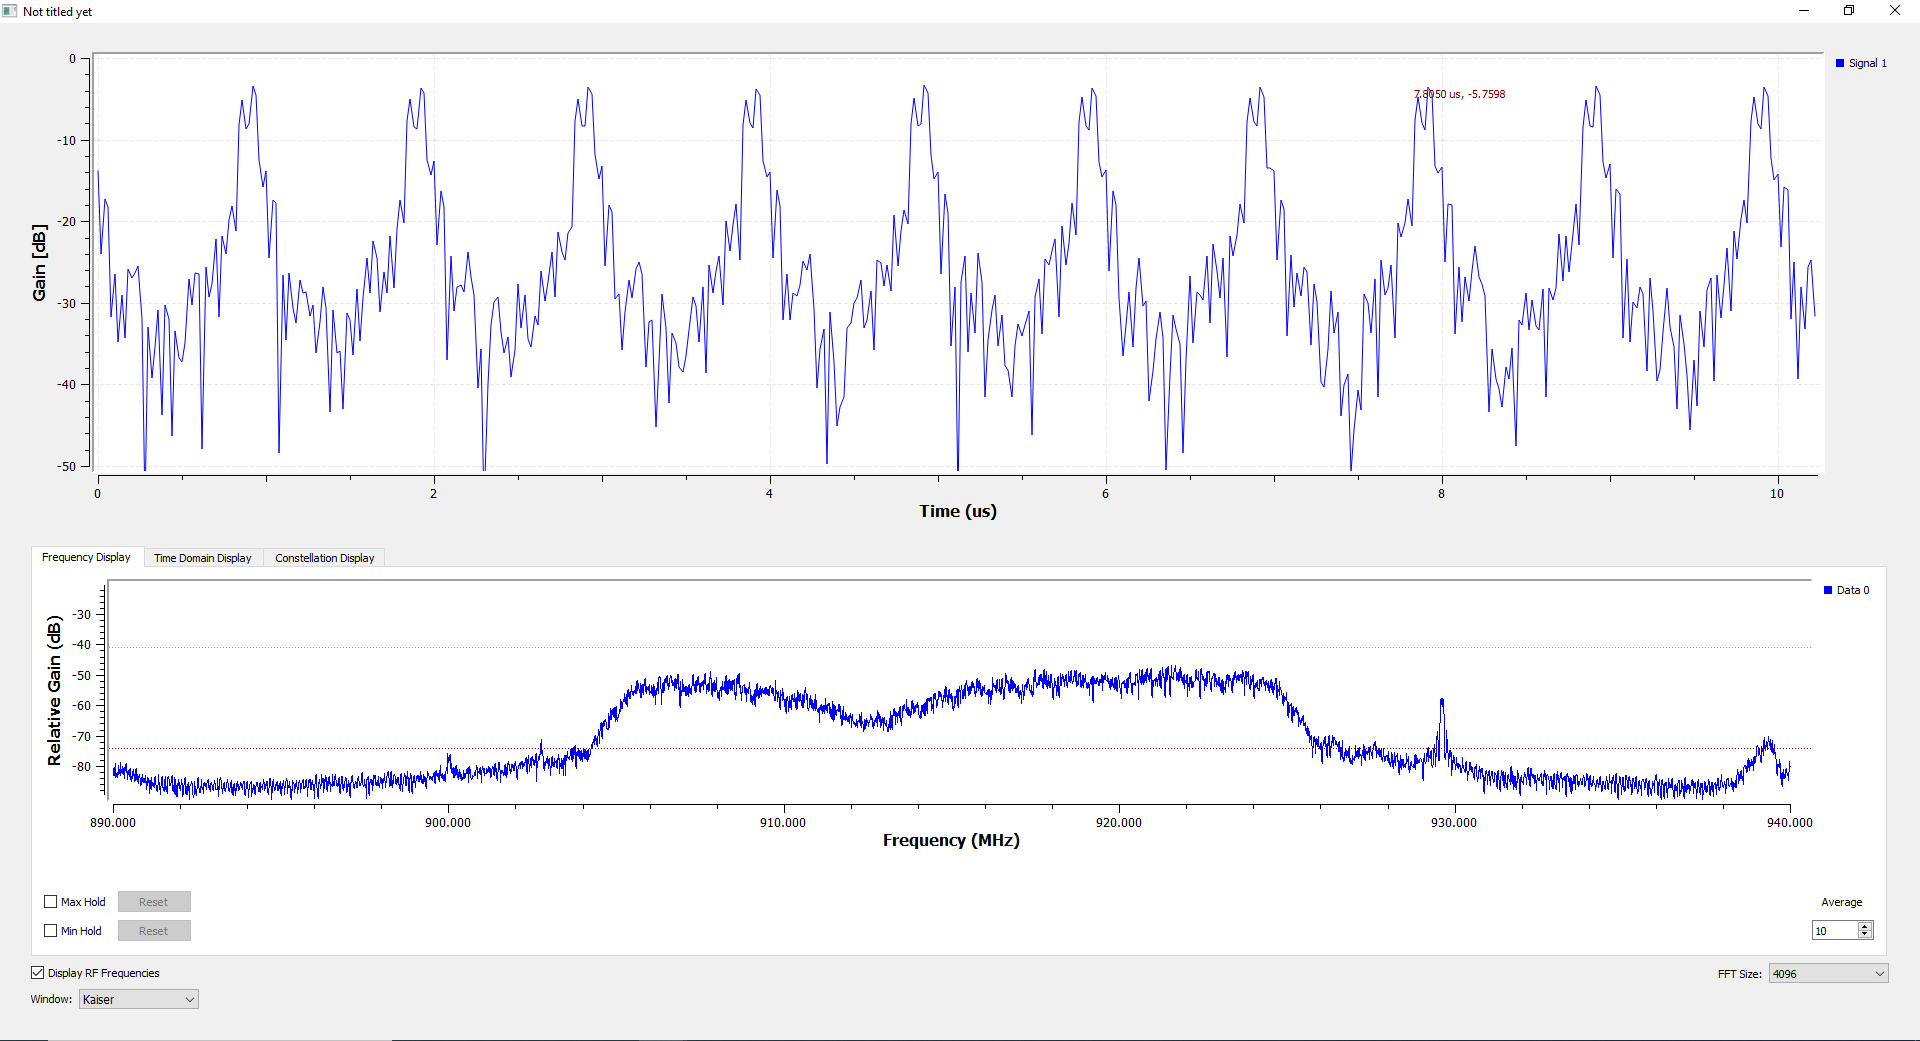
\includegraphics[width=\textwidth]{selective_fading.PNG}
\caption{Frequency-Selective Fading.}
\label{fig:selective_fading}
\end{figure}

\subsection{Flat Fading}
\begin{figure}[H]
\centering
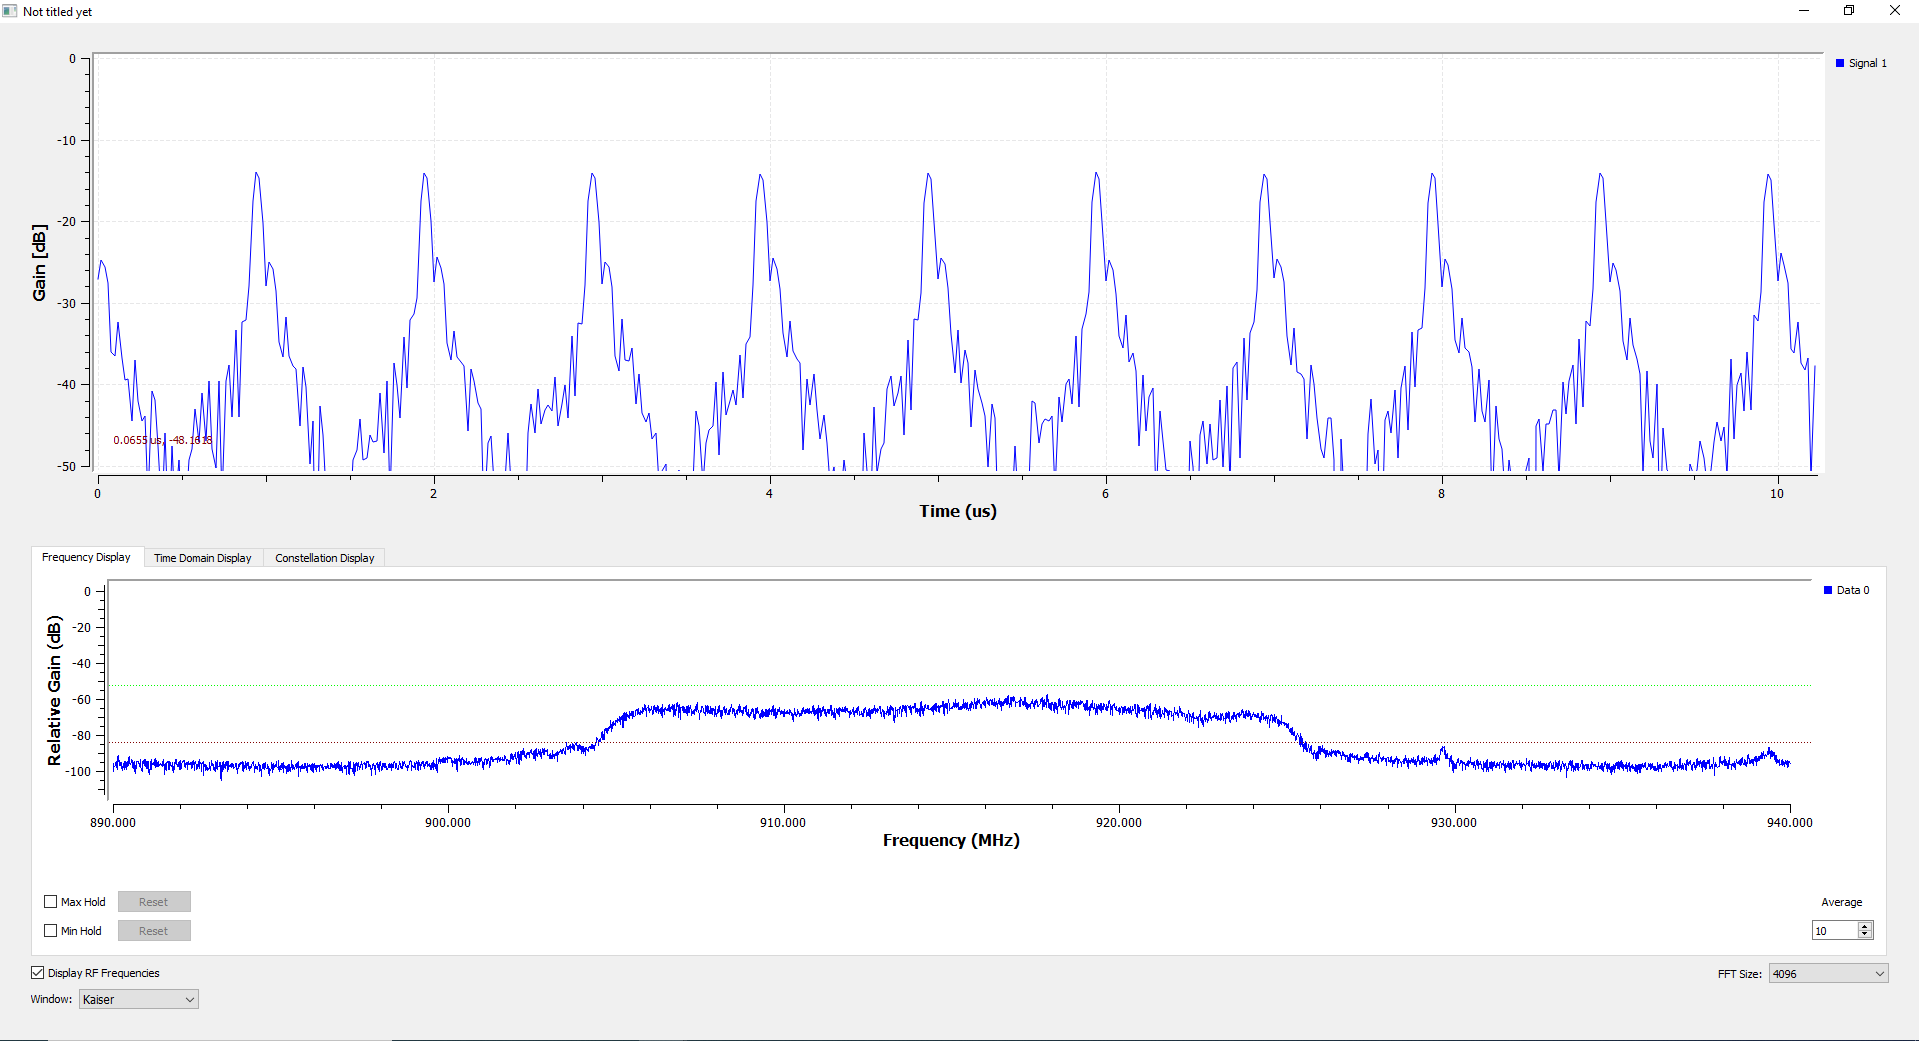
\includegraphics[width=\textwidth]{flat_fading.PNG}
\caption{Flat Fading.}
\label{fig:flat_fading}
\end{figure}

\subsection{Channel Frequency Response}
\begin{figure}[H]
\centering
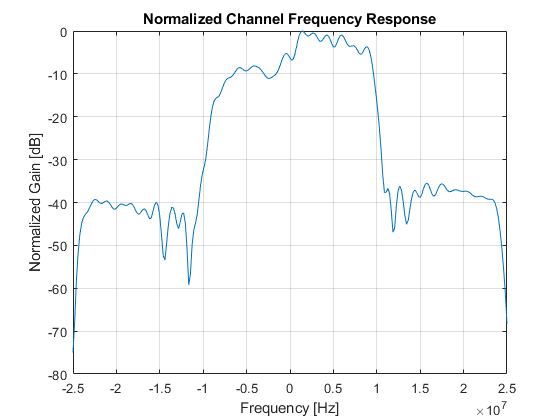
\includegraphics[width=\textwidth]{CFR.png}
\caption{Channel Frequency Response.}
\label{fig:CFR}
\end{figure}

\subsection{Channel Impulse Response for 30 Pulses}
\begin{figure}[H]
\centering
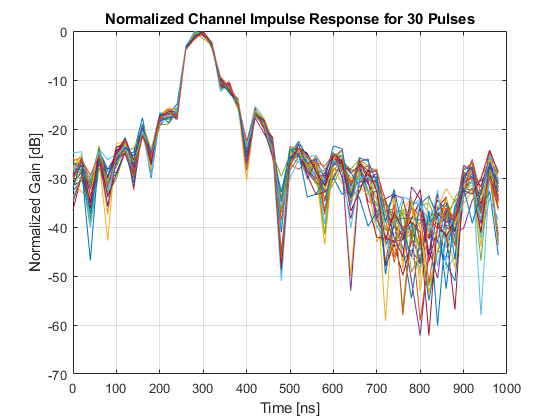
\includegraphics[width=\textwidth]{CIR_ALL.png}
\caption{Channel Impulse Response for 30 Pulses.}
\label{fig:CIR_ALL}
\end{figure}

\subsection{Average Normalized Channel Impulse Response}
\begin{figure}[H]
\centering
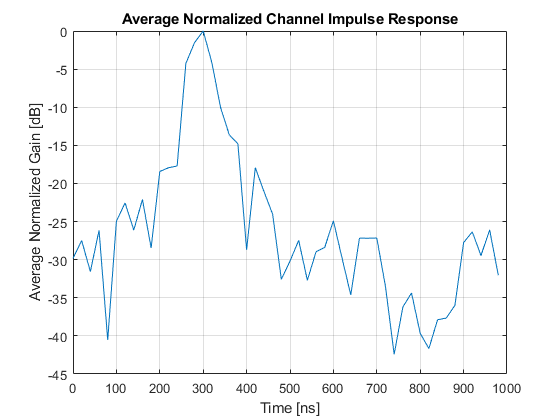
\includegraphics[width=\textwidth]{CIR_AVG.png}
\caption{Average Normalized Channel Impulse Response.}
\label{fig:CIR_AVG}
\end{figure}

\subsection{Normalized Correlation}
\begin{figure}[H]
\centering
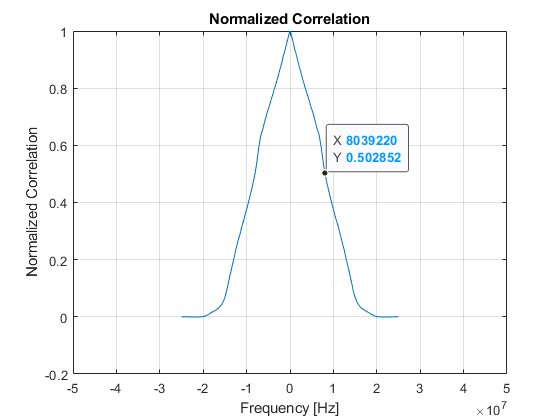
\includegraphics[width=\textwidth]{correlation.png}
\caption{Normalized Correlation.}
\label{fig:correlation}
\end{figure}

\section{Discussion}
The data from both the omni-directional and directional antennas provided comprehensive insight into the channel's behavior under different fading conditions. The results were consistent with theoretical expectations and demonstrated the practical implications for wireless communication systems, especially in environments prone to multi-path fading. The Coherence Bandwidth was found to be 8.039 MHz from the Normalized Correlation plot.

\section{MATLAB Code}
The MATLAB code for the transmitter and the scripts for CIR/CFR generation are detailed in the appendices. These scripts were vital in processing the collected data and generating the plots used for analysis.

\section{Conclusion}
The experiment successfully demonstrated the effects of frequency-selective and flat fading using omni-directional and directional antennas. The findings have significant implications for the design and deployment of wireless communication systems, particularly in complex environments.


\newpage
\section{Doppler Shift Calculation and Fan Speed Estimation}

The Doppler effect is a phenomenon observed when there is a relative motion between a wave source and an observer. In the context of radar systems, the Doppler effect causes a shift in the frequency of the reflected waves when there is relative motion between the radar and the target object. This shift in frequency, known as the Doppler shift, can be used to calculate the velocity of the target object.

To determine the Doppler shift, we utilize a software-defined radio (SDR) to transmit and receive signals. The following MATLAB code snippet outlines the process of generating a continuous wave (CW) tone, transmitting it, and analyzing the received signal to determine the frequency shift.

\subsection{Code Overview}

The code starts by setting up the basic parameters such as the sampling frequency (\texttt{fsample}), the carrier frequency (\texttt{fc}), and the duration of the transmitted packet (\texttt{Tpacket}). The number of samples (\texttt{Nsamples}) is derived from the product of \texttt{Tpacket} and \texttt{fsample}. A time vector (\texttt{t}) is created, and a CW tone at a specified frequency (\texttt{frequencyTone}) is generated as the IQ data (\texttt{IQdataTX}).

Normalization of the IQ data is performed to ensure that the maximum absolute value is less than 1, which is a requirement for the operation of remote SDRs. This step is crucial to avoid clipping and potential distortion in the transmitted signal.

Next, the code includes a function call to \texttt{analyzeIQdata}, which is responsible for visualizing the time domain signal, its power spectral density, and other properties of the transmitted IQ data.

Finally, the transmission of the signal is set up via a Pluto SDR with specified parameters like radio ID, gain, center frequency, and baseband sample rate. The function \texttt{transmitRepeat} is used to continuously transmit the generated IQ data.

\subsection{Determining the Doppler Shift}

The transmitted CW tone reflects off moving objects, and the received signal is analyzed to measure the frequency shift. By comparing the frequency of the transmitted tone and the frequency of the received signal, we can calculate the Doppler shift. This shift, when applied to the Doppler shift equations, allows us to determine the velocity of the object in motion relative to the radar.

Using the Doppler effect, we can deduce not only the presence of an object but also its speed and direction of movement, which are vital parameters in radar technology for applications such as traffic monitoring, autonomous vehicles, and airspace surveillance.
\subsection{The Math}
The velocity \( v \) of the fan blades is calculated using the Doppler shift equation:
\[
f_d = \frac{v \cos(\theta)}{c} f_c
\]
where:
\begin{itemize}
    \item \( f_d \) is the Doppler shift,
    \item \( v \) is the velocity of the object,
    \item \( c \) is the speed of light (\(3 \times 10^8\) m/s),
    \item \( f_c \) is the carrier frequency,
    \item \( \theta \) is the angle between the motion of the object and the line-of-sight of the observer.
\end{itemize}

For the maximum velocity, where \( \theta = 0 \) or \( \theta = 180 \) degrees, \( \cos(\theta) = 1 \), the Doppler shift equation simplifies to:
\[
v = \frac{\Delta f c}{f_c}
\]

The frequency shifts \( \Delta f_{\text{right}} \) and \( \Delta f_{\text{left}} \) are the differences in frequency on the right and left side of the center frequency. These shifts are used to calculate the velocities \( v_1 \) and \( v_2 \):
\[
v_1 = \frac{\Delta f_{\text{right}} c}{f_c} = \frac{(86.95 \text{ kHz} - 85.8 \text{ kHz}) \cdot 3 \times 10^8}{5.9 \times 10^9 + 100 \times 10^3} \approx 62.54 \text{ m/s}
\]
\[
v_2 = \frac{\Delta f_{\text{left}} c}{f_c} = \frac{(85.8 \text{ kHz} - 84.49 \text{ kHz}) \cdot 3 \times 10^8}{5.9 \times 10^9 + 100 \times 10^3} \approx 62.54 \text{ m/s}
\]

The average velocity \( v \) is then calculated as:
\[
v = \frac{v_1 + v_2}{2} \approx 62.54 \text{ m/s}
\]

To find the revolutions per minute (RPM), the linear velocity is converted to angular velocity and then to RPM:
\[
\text{RPM} = \frac{v}{2 \pi r} \times 60
\]

Given the blade radius \( r = 0.27 \) m, the RPM is calculated for both velocities \( v_1 \) and \( v_2 \), and the average RPM is taken as:
\[
\text{RPM} = \frac{\text{RPM}_1 + \text{RPM}_2}{2} \approx \frac{2068.08 + 2355.81}{2} \approx 2211.95 \text{ RPM}
\]


\section*{Spectral Analysis Images}

\subsection*{Pure Tone without Fan}
\begin{figure}[H]
    \centering
    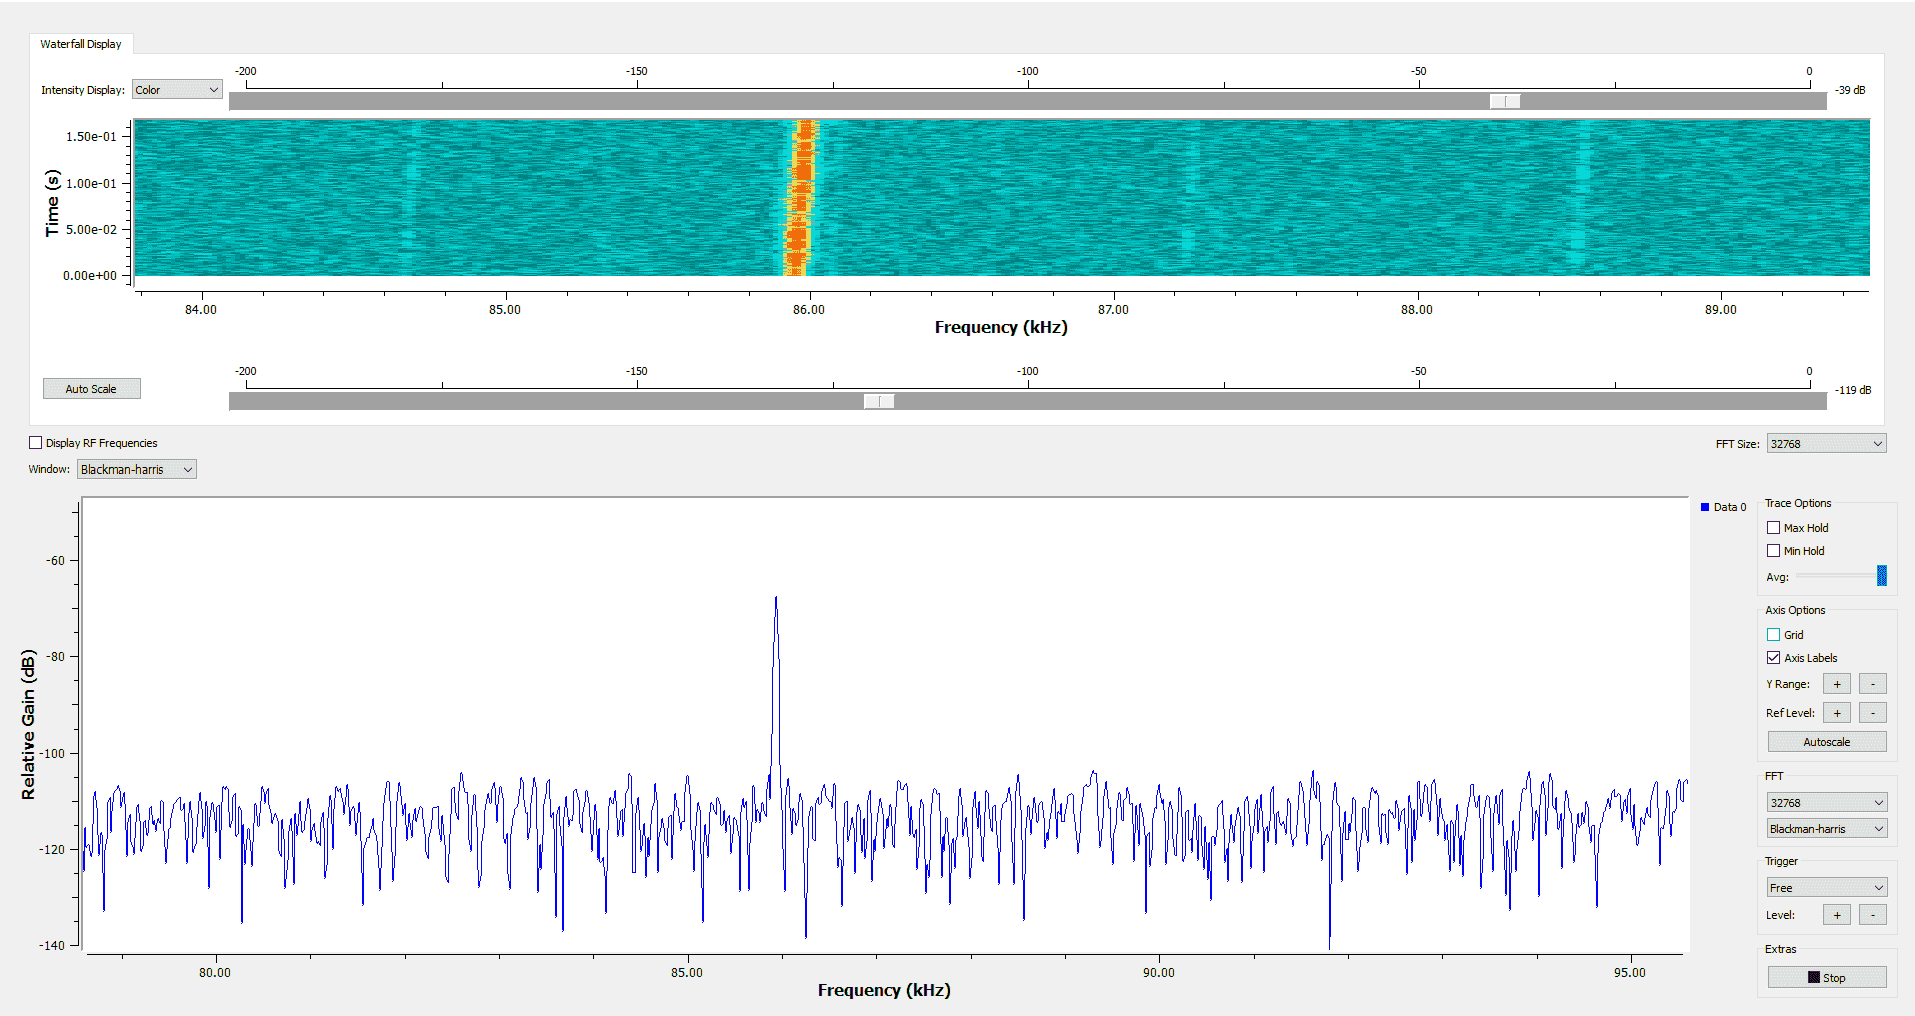
\includegraphics[width=\textwidth]{no_fan.png}
    \caption{Spectrum with no fan interference.}
    \label{fig:no_fan}
\end{figure}

\subsection*{Fan at High Speed}
\begin{figure}[H]
    \centering
    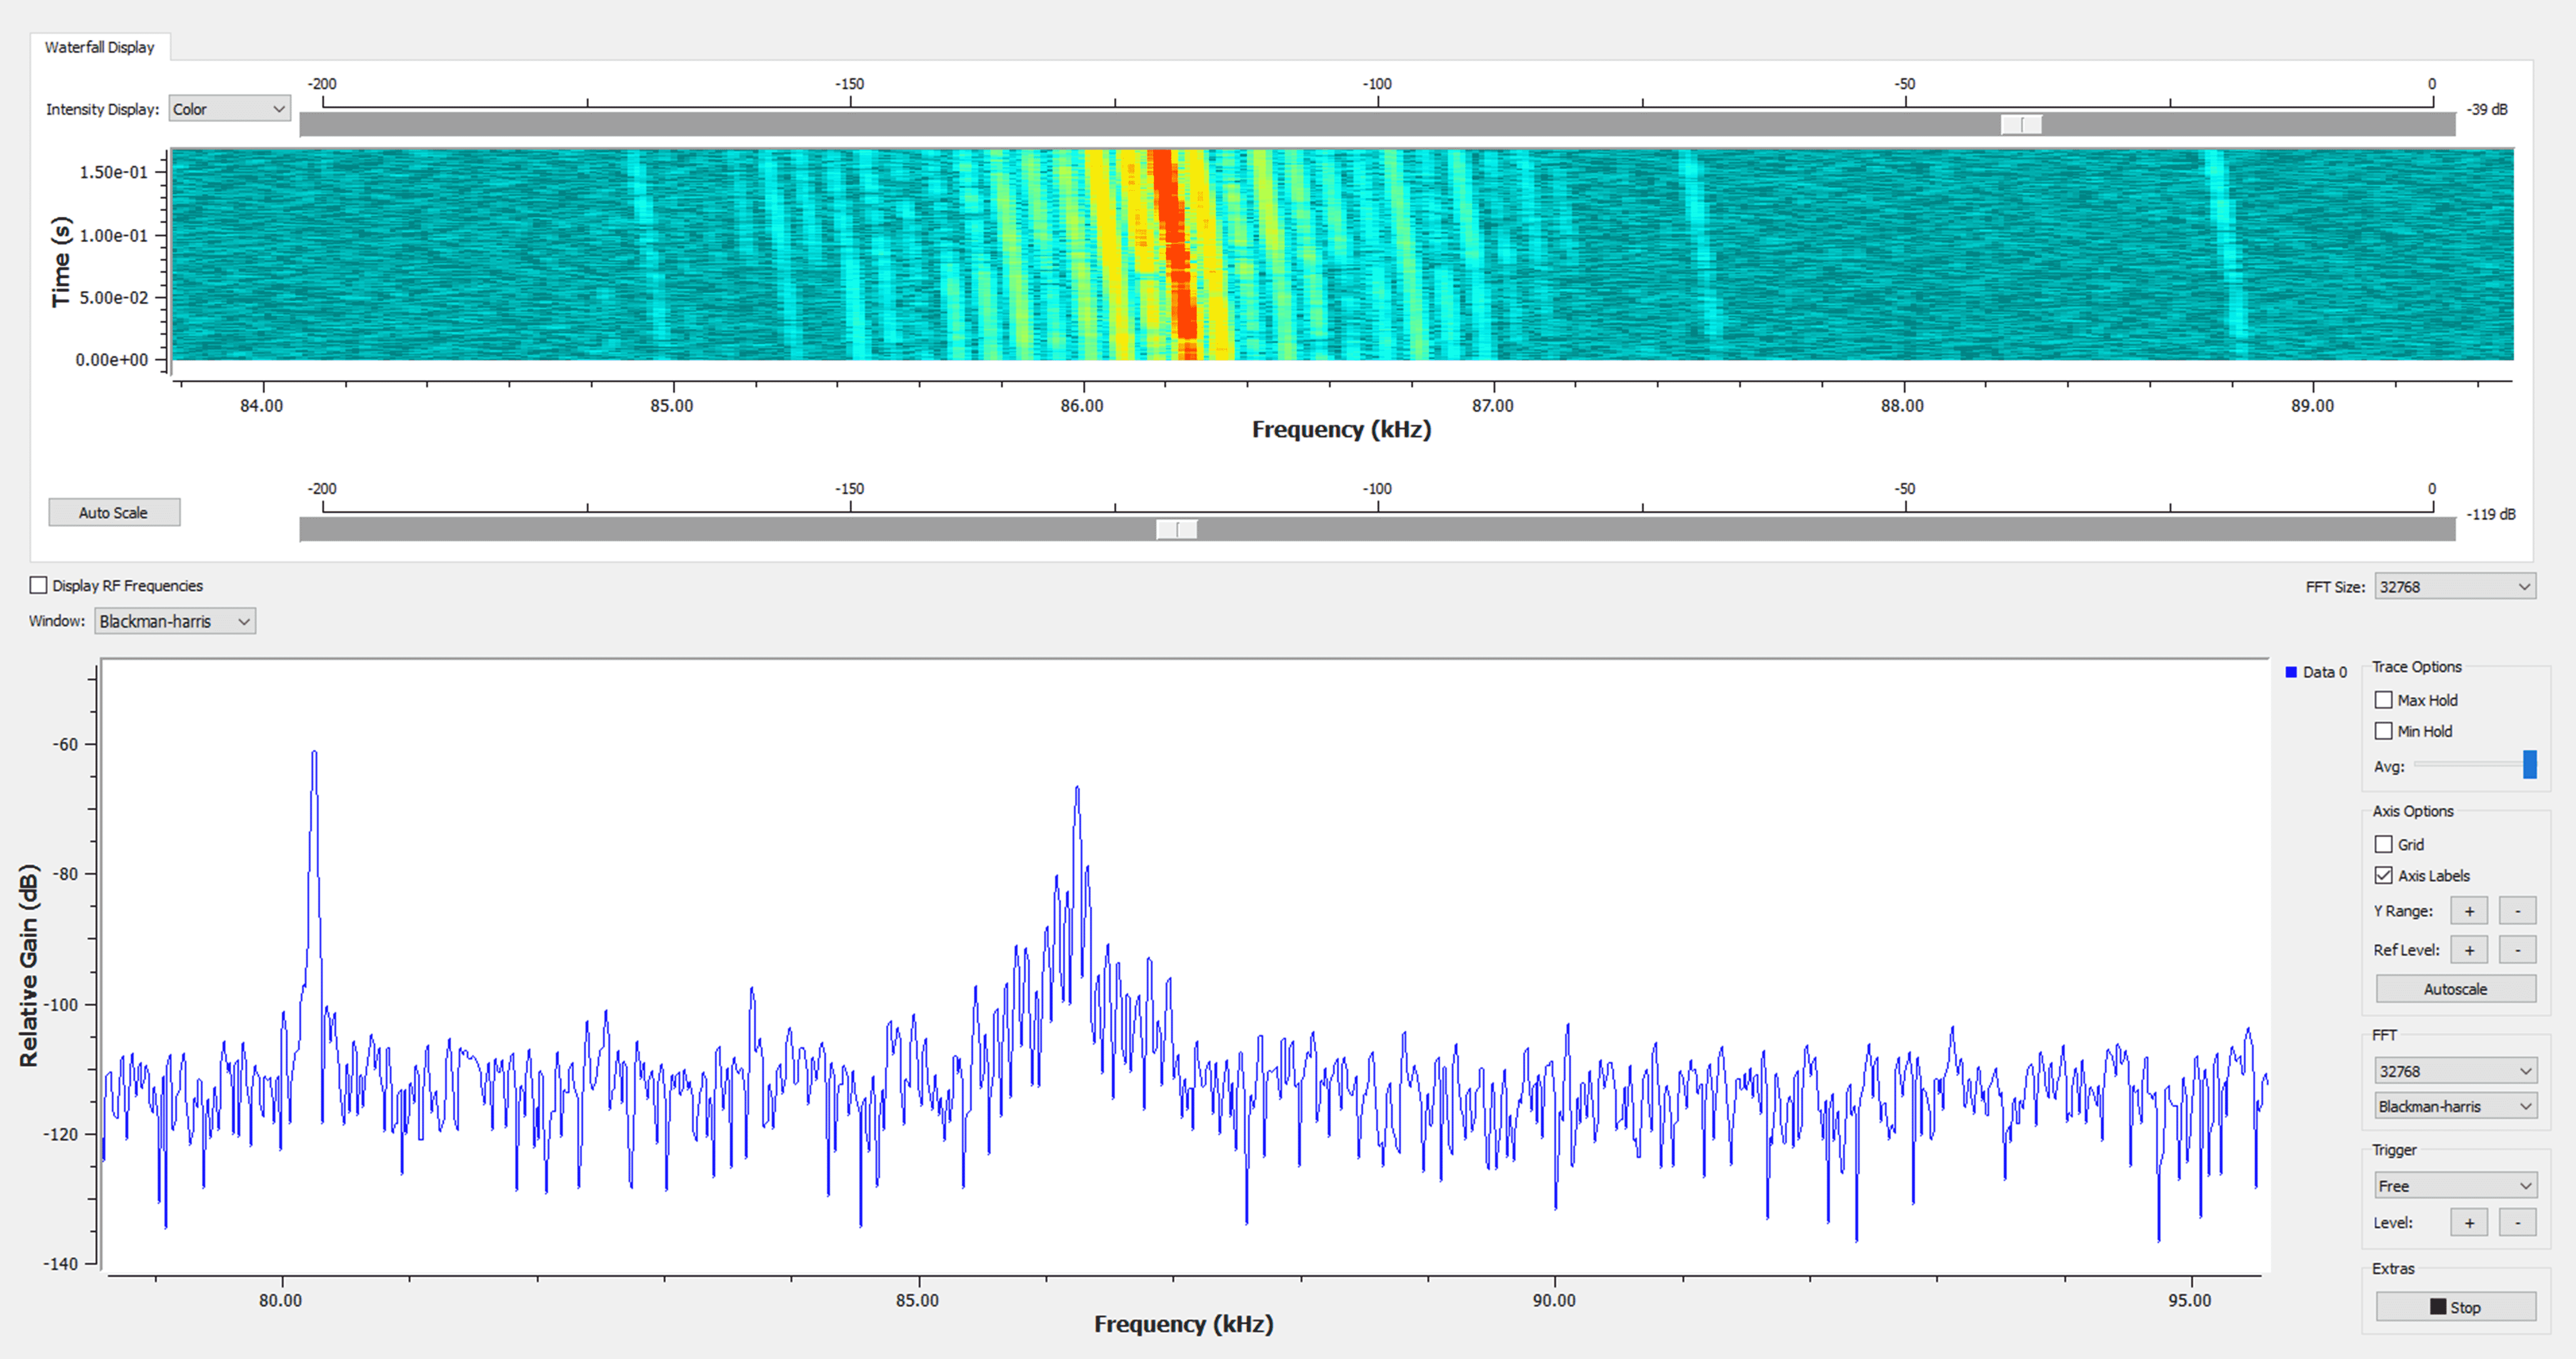
\includegraphics[width=\textwidth]{fan_high.png}
    \caption{Spectrum with the fan at high speed.}
    \label{fig:fan_high}
\end{figure}

\subsection*{Fan High to Off Transition}
\begin{figure}[H]
    \centering
    \includegraphics[width=\textwidth]{fan_high_to_off.png}
    \caption{Spectrum during the transition from high to off.}
    \label{fig:fan_high_to_off}
\end{figure}

\subsection*{Fan at Low Speed}
\begin{figure}[H]
    \centering
    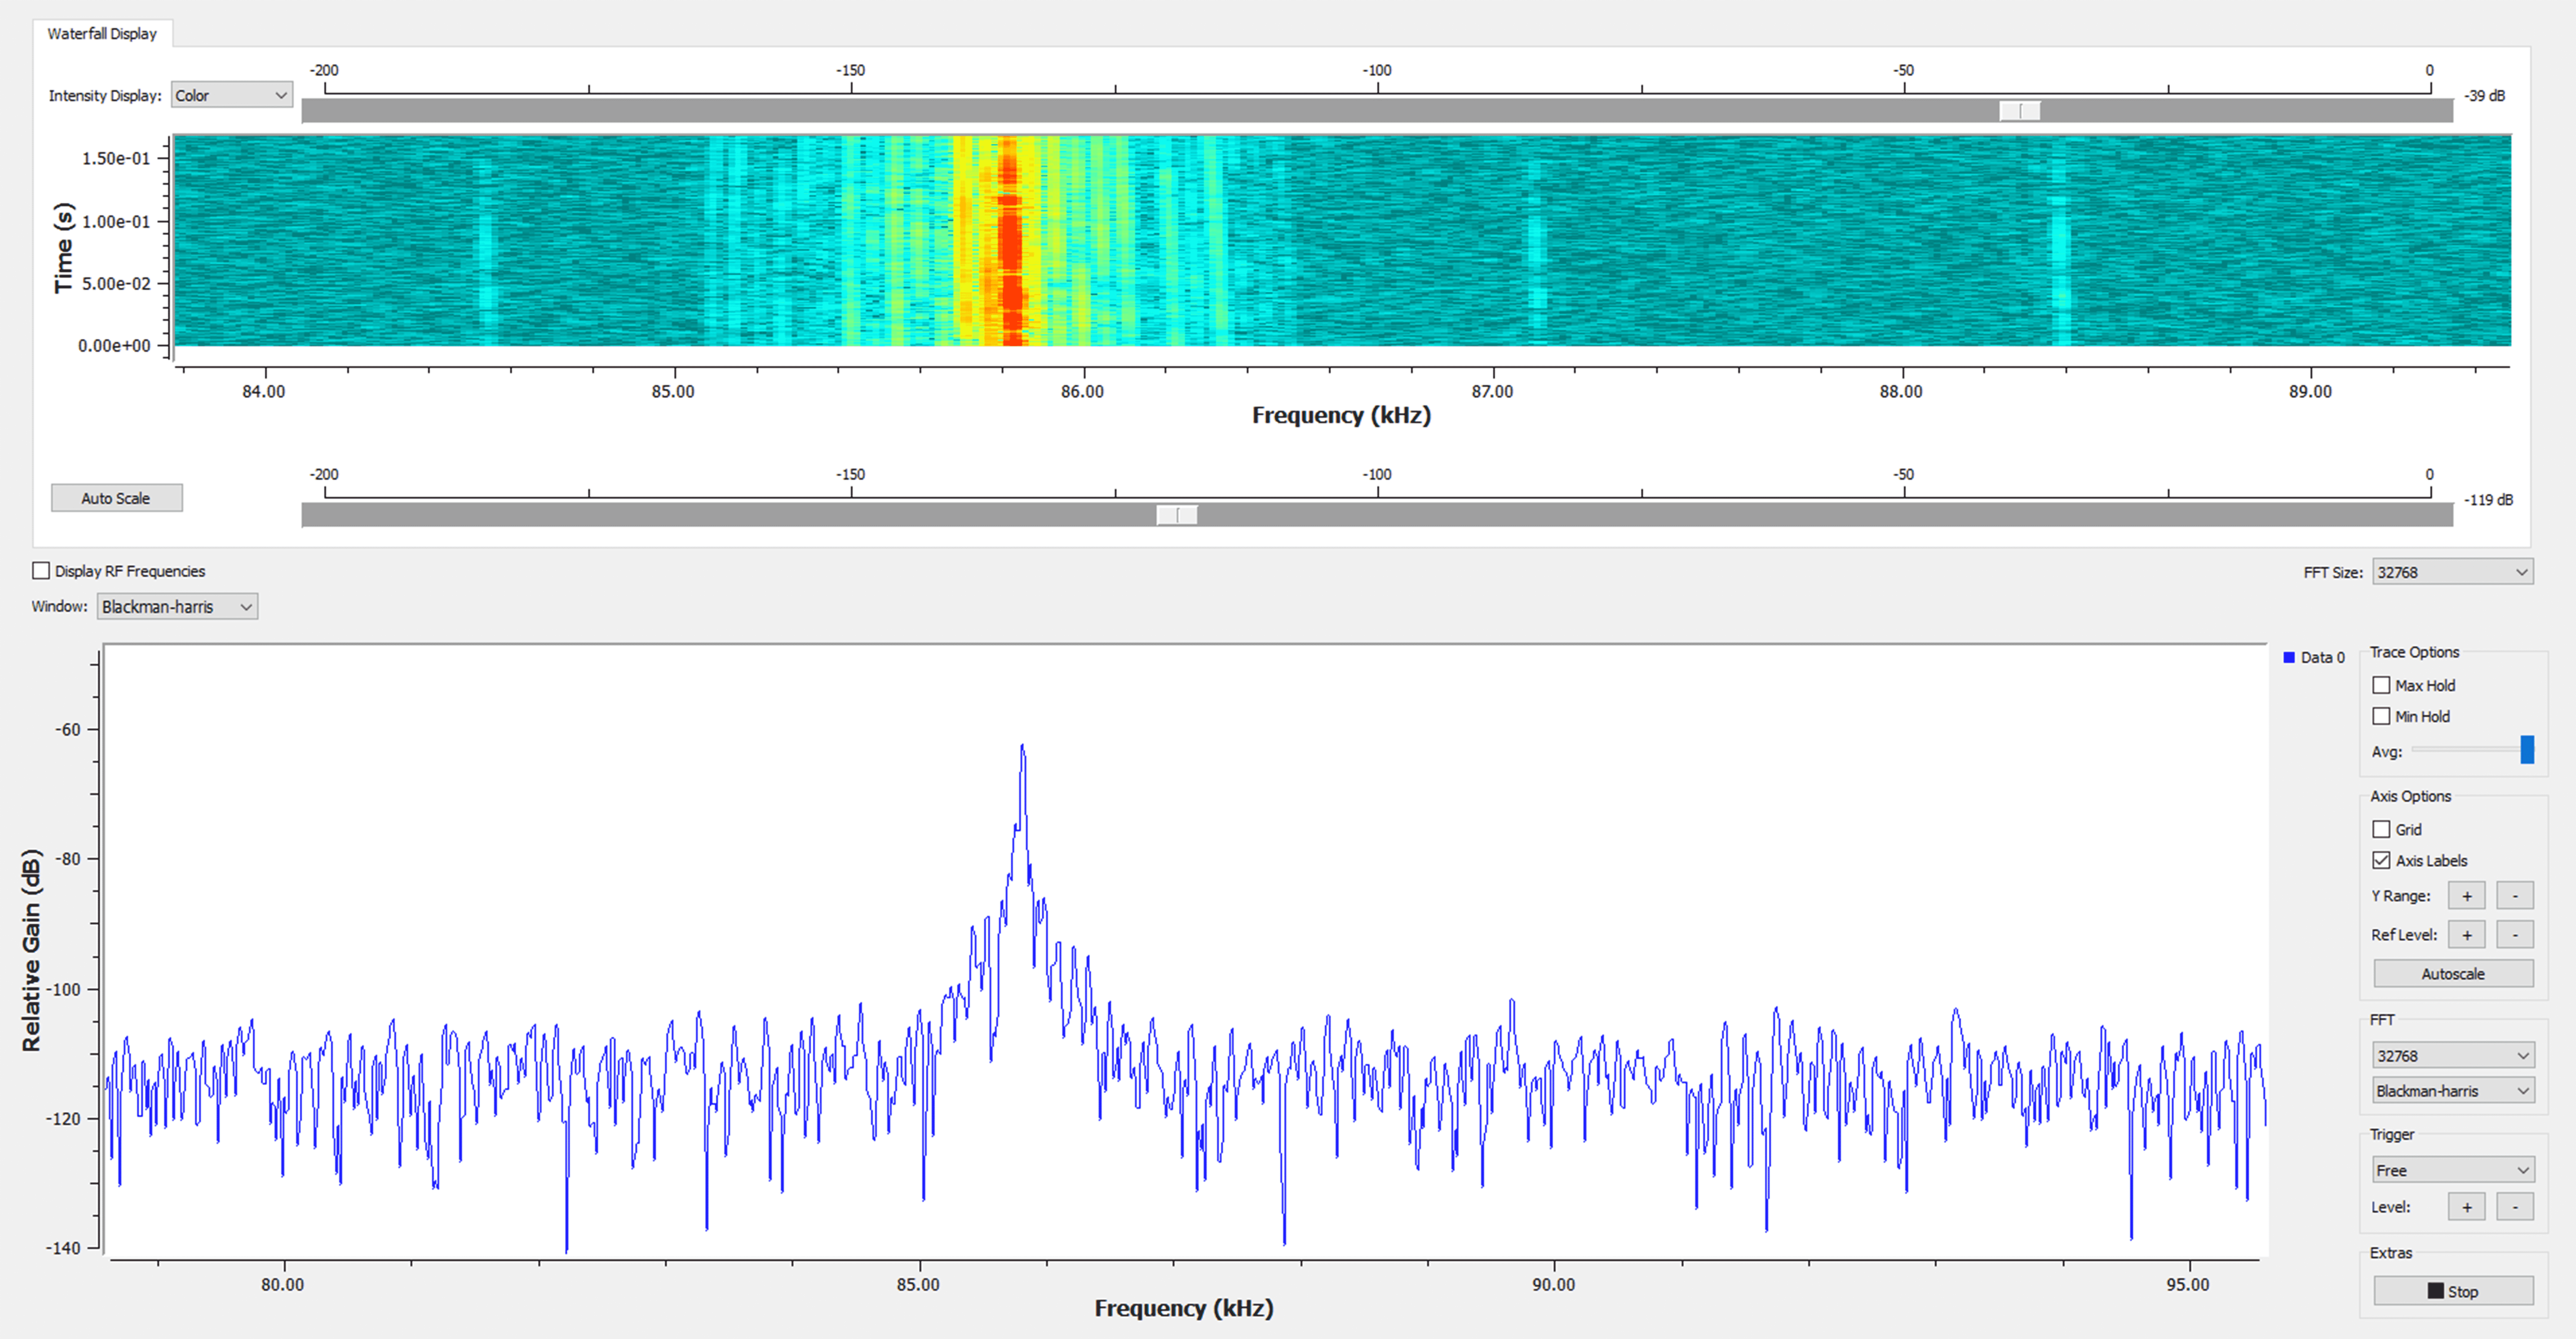
\includegraphics[width=\textwidth]{Fan_low.png}
    \caption{Spectrum with the fan at low speed.}
    \label{fig:fan_low}
\end{figure}

\subsection*{Fan Low to Medium Transition}
\begin{figure}[H]
    \centering
    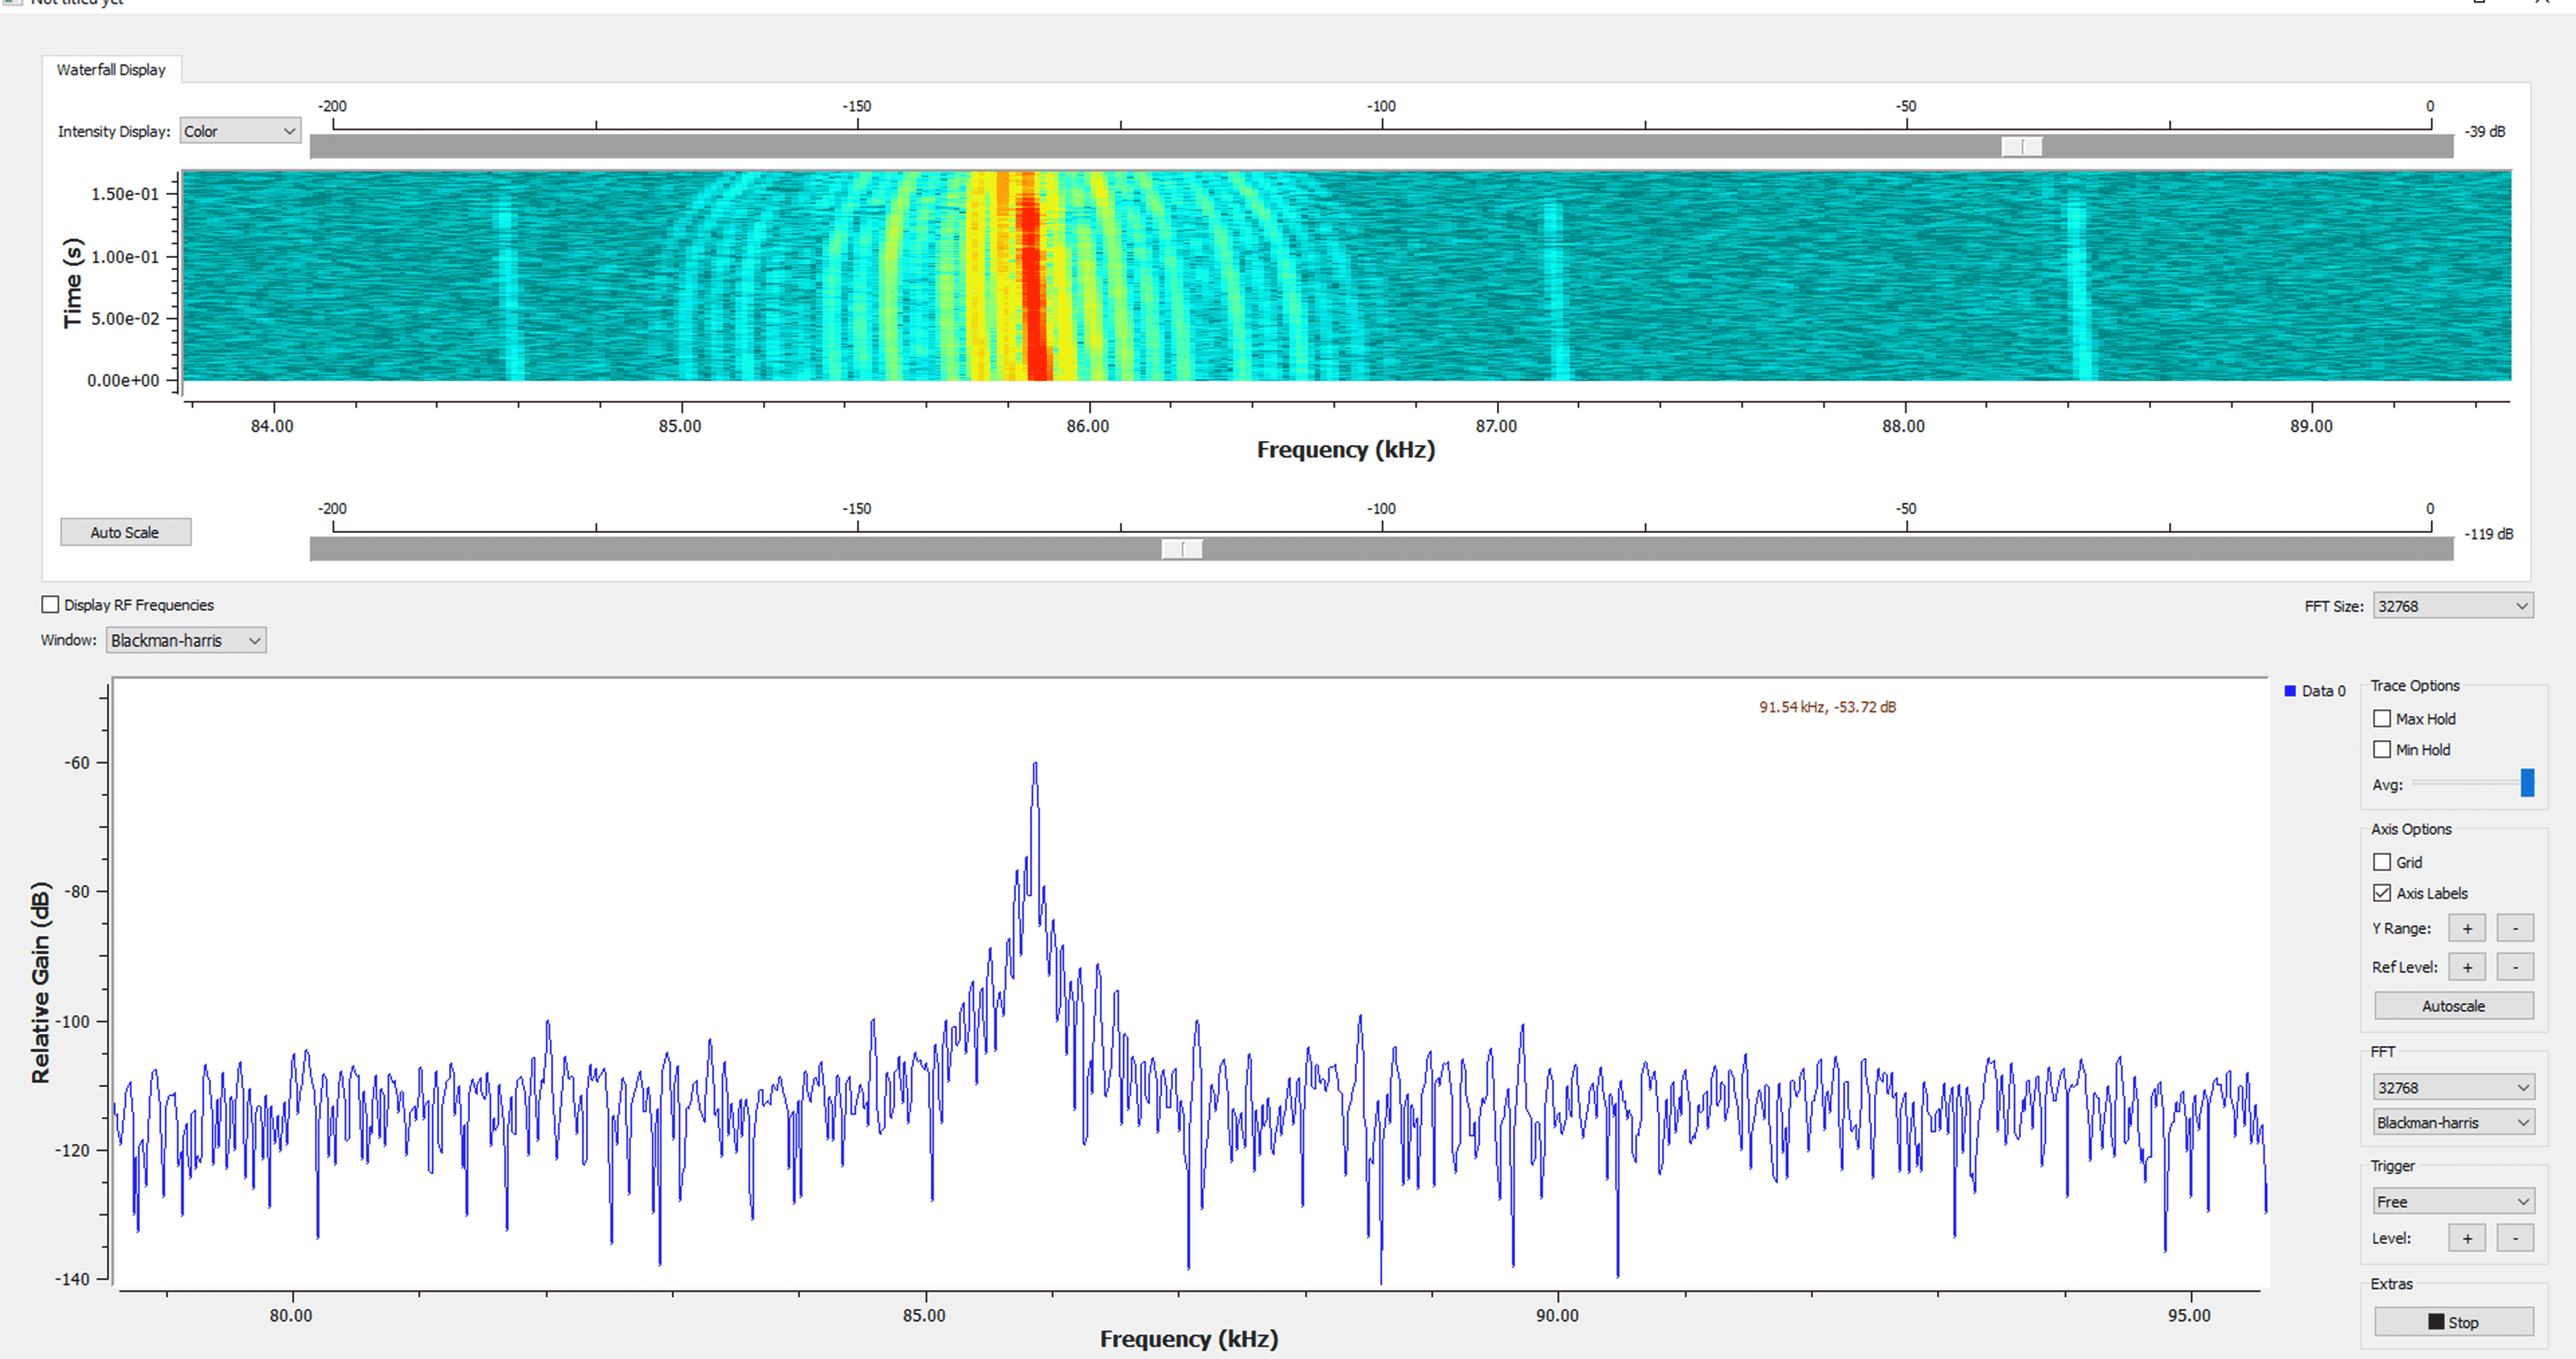
\includegraphics[width=\textwidth]{fan_low_to_medium.png}
    \caption{Spectrum during the transition from low to medium.}
    \label{fig:fan_low_to_medium}
\end{figure}

\subsection*{Fan Medium to High Transition}
\begin{figure}[H]
    \centering
    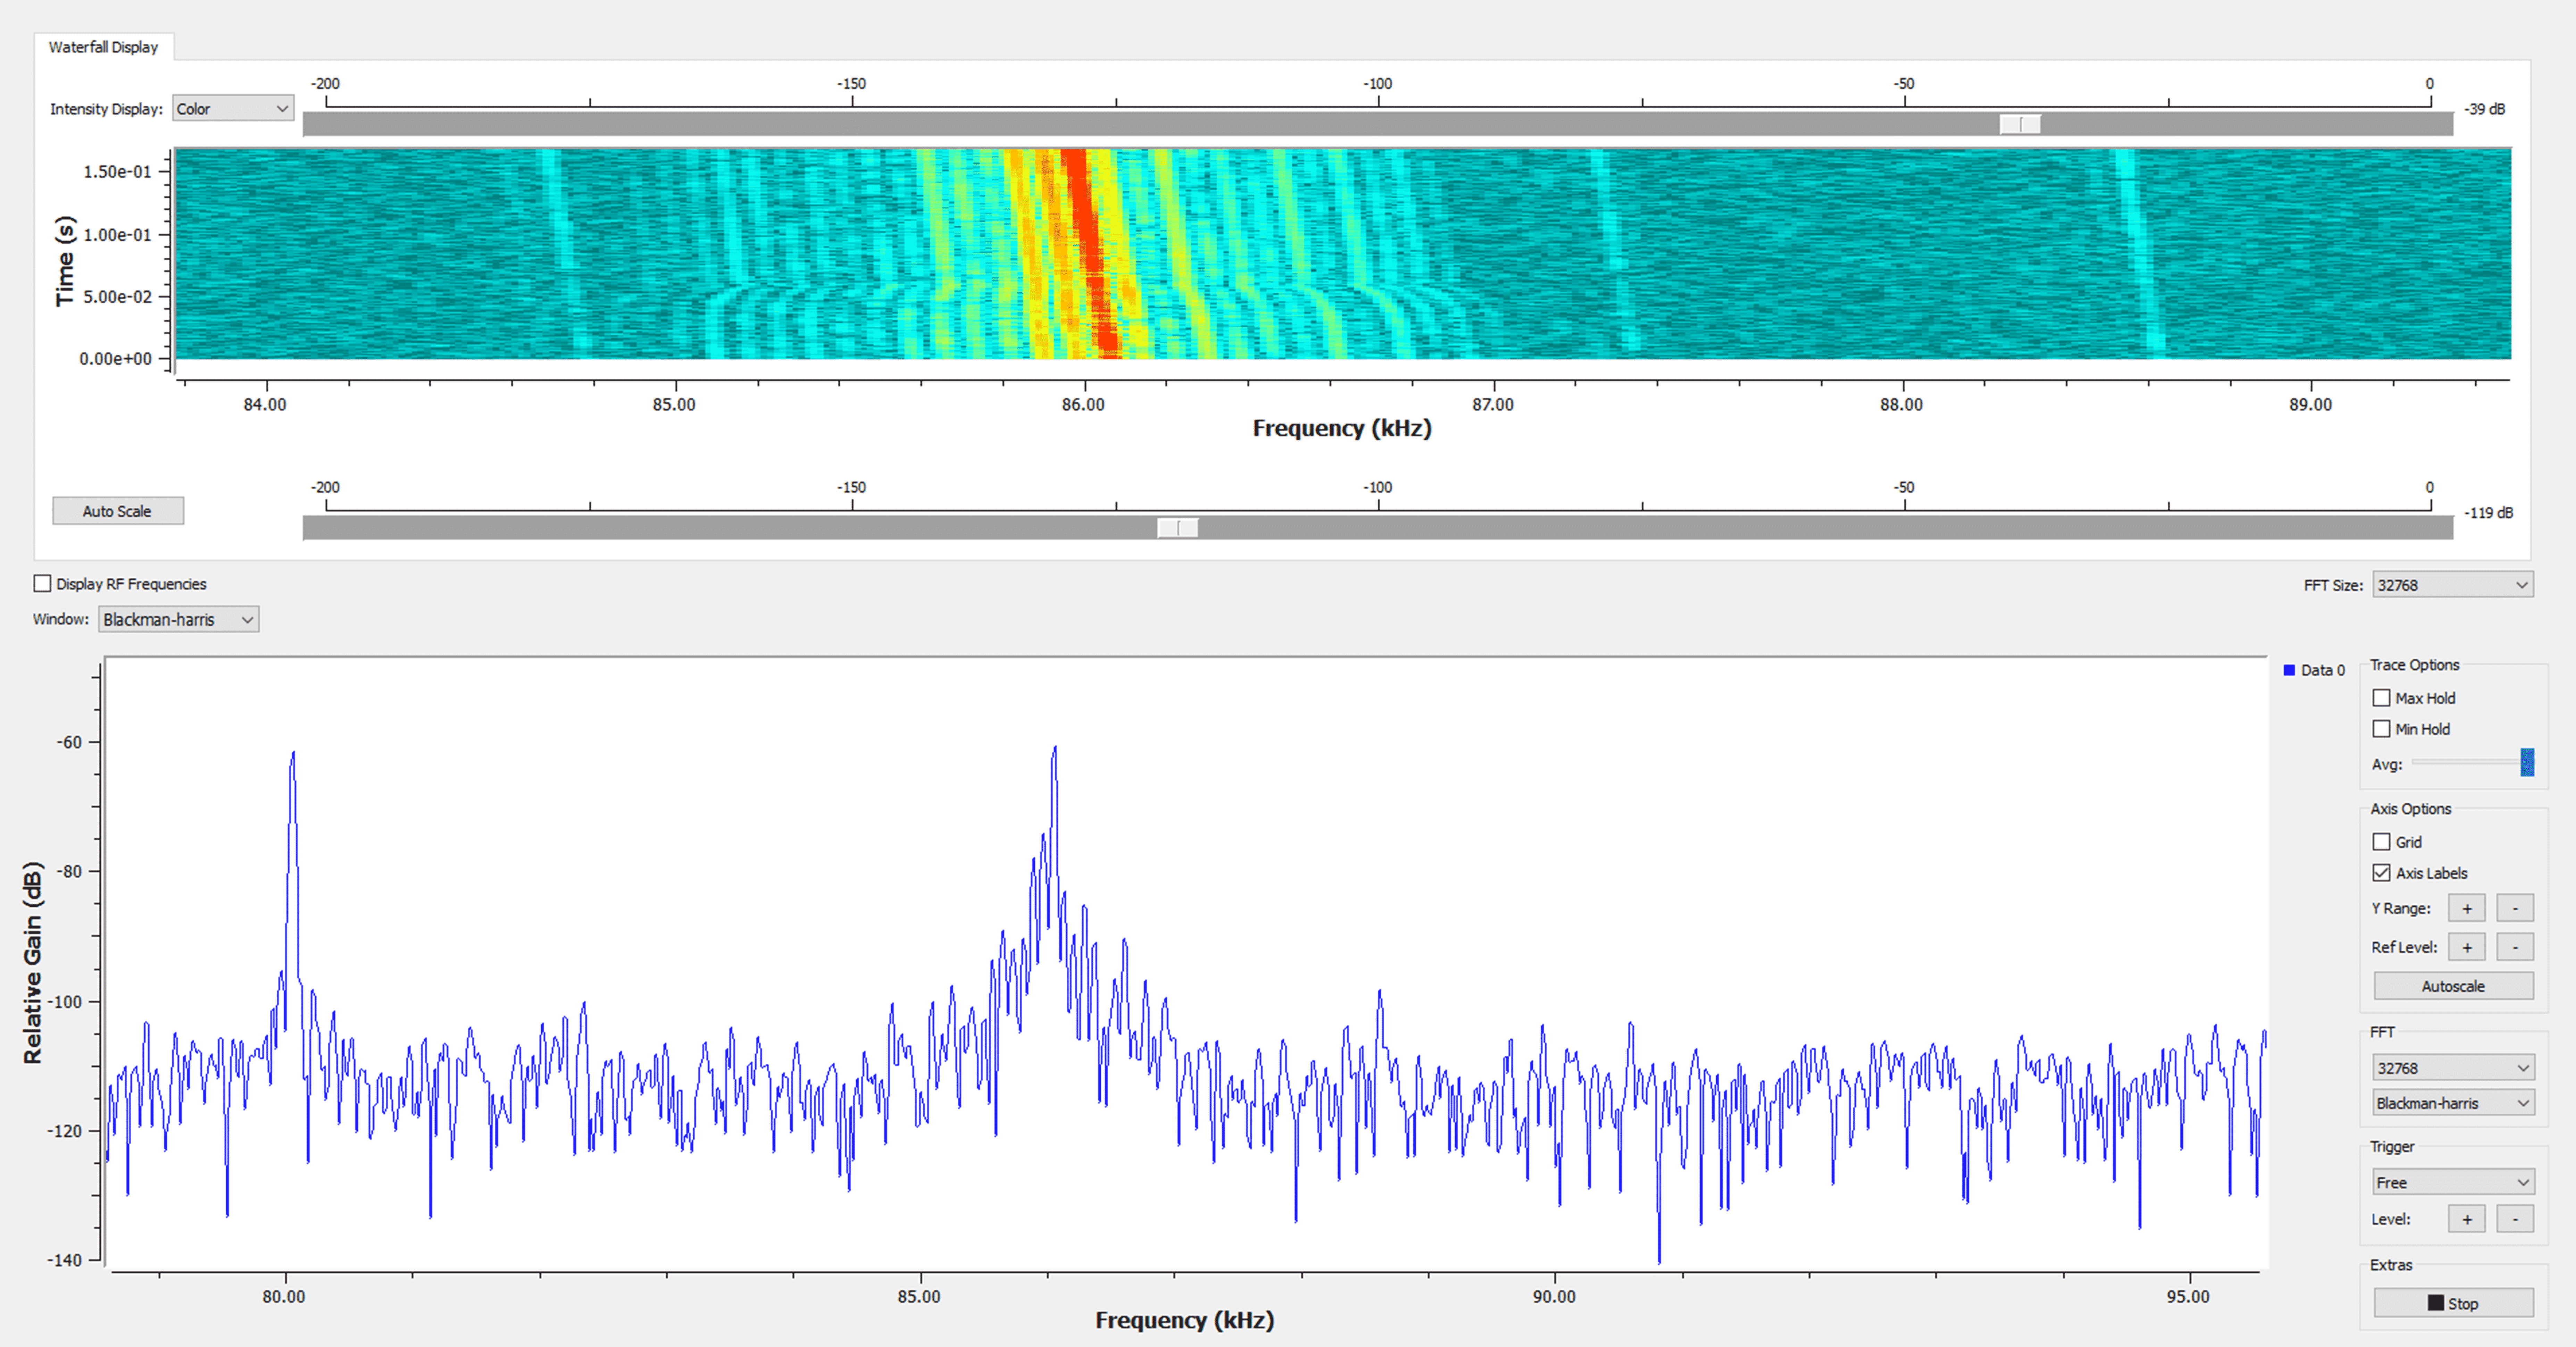
\includegraphics[width=\textwidth]{fan_med_to_high.png}
    \caption{Spectrum during the transition from medium to high.}
    \label{fig:fan_med_to_high}
\end{figure}

\subsection*{Fan Off to High Transition}
\begin{figure}[H]
    \centering
    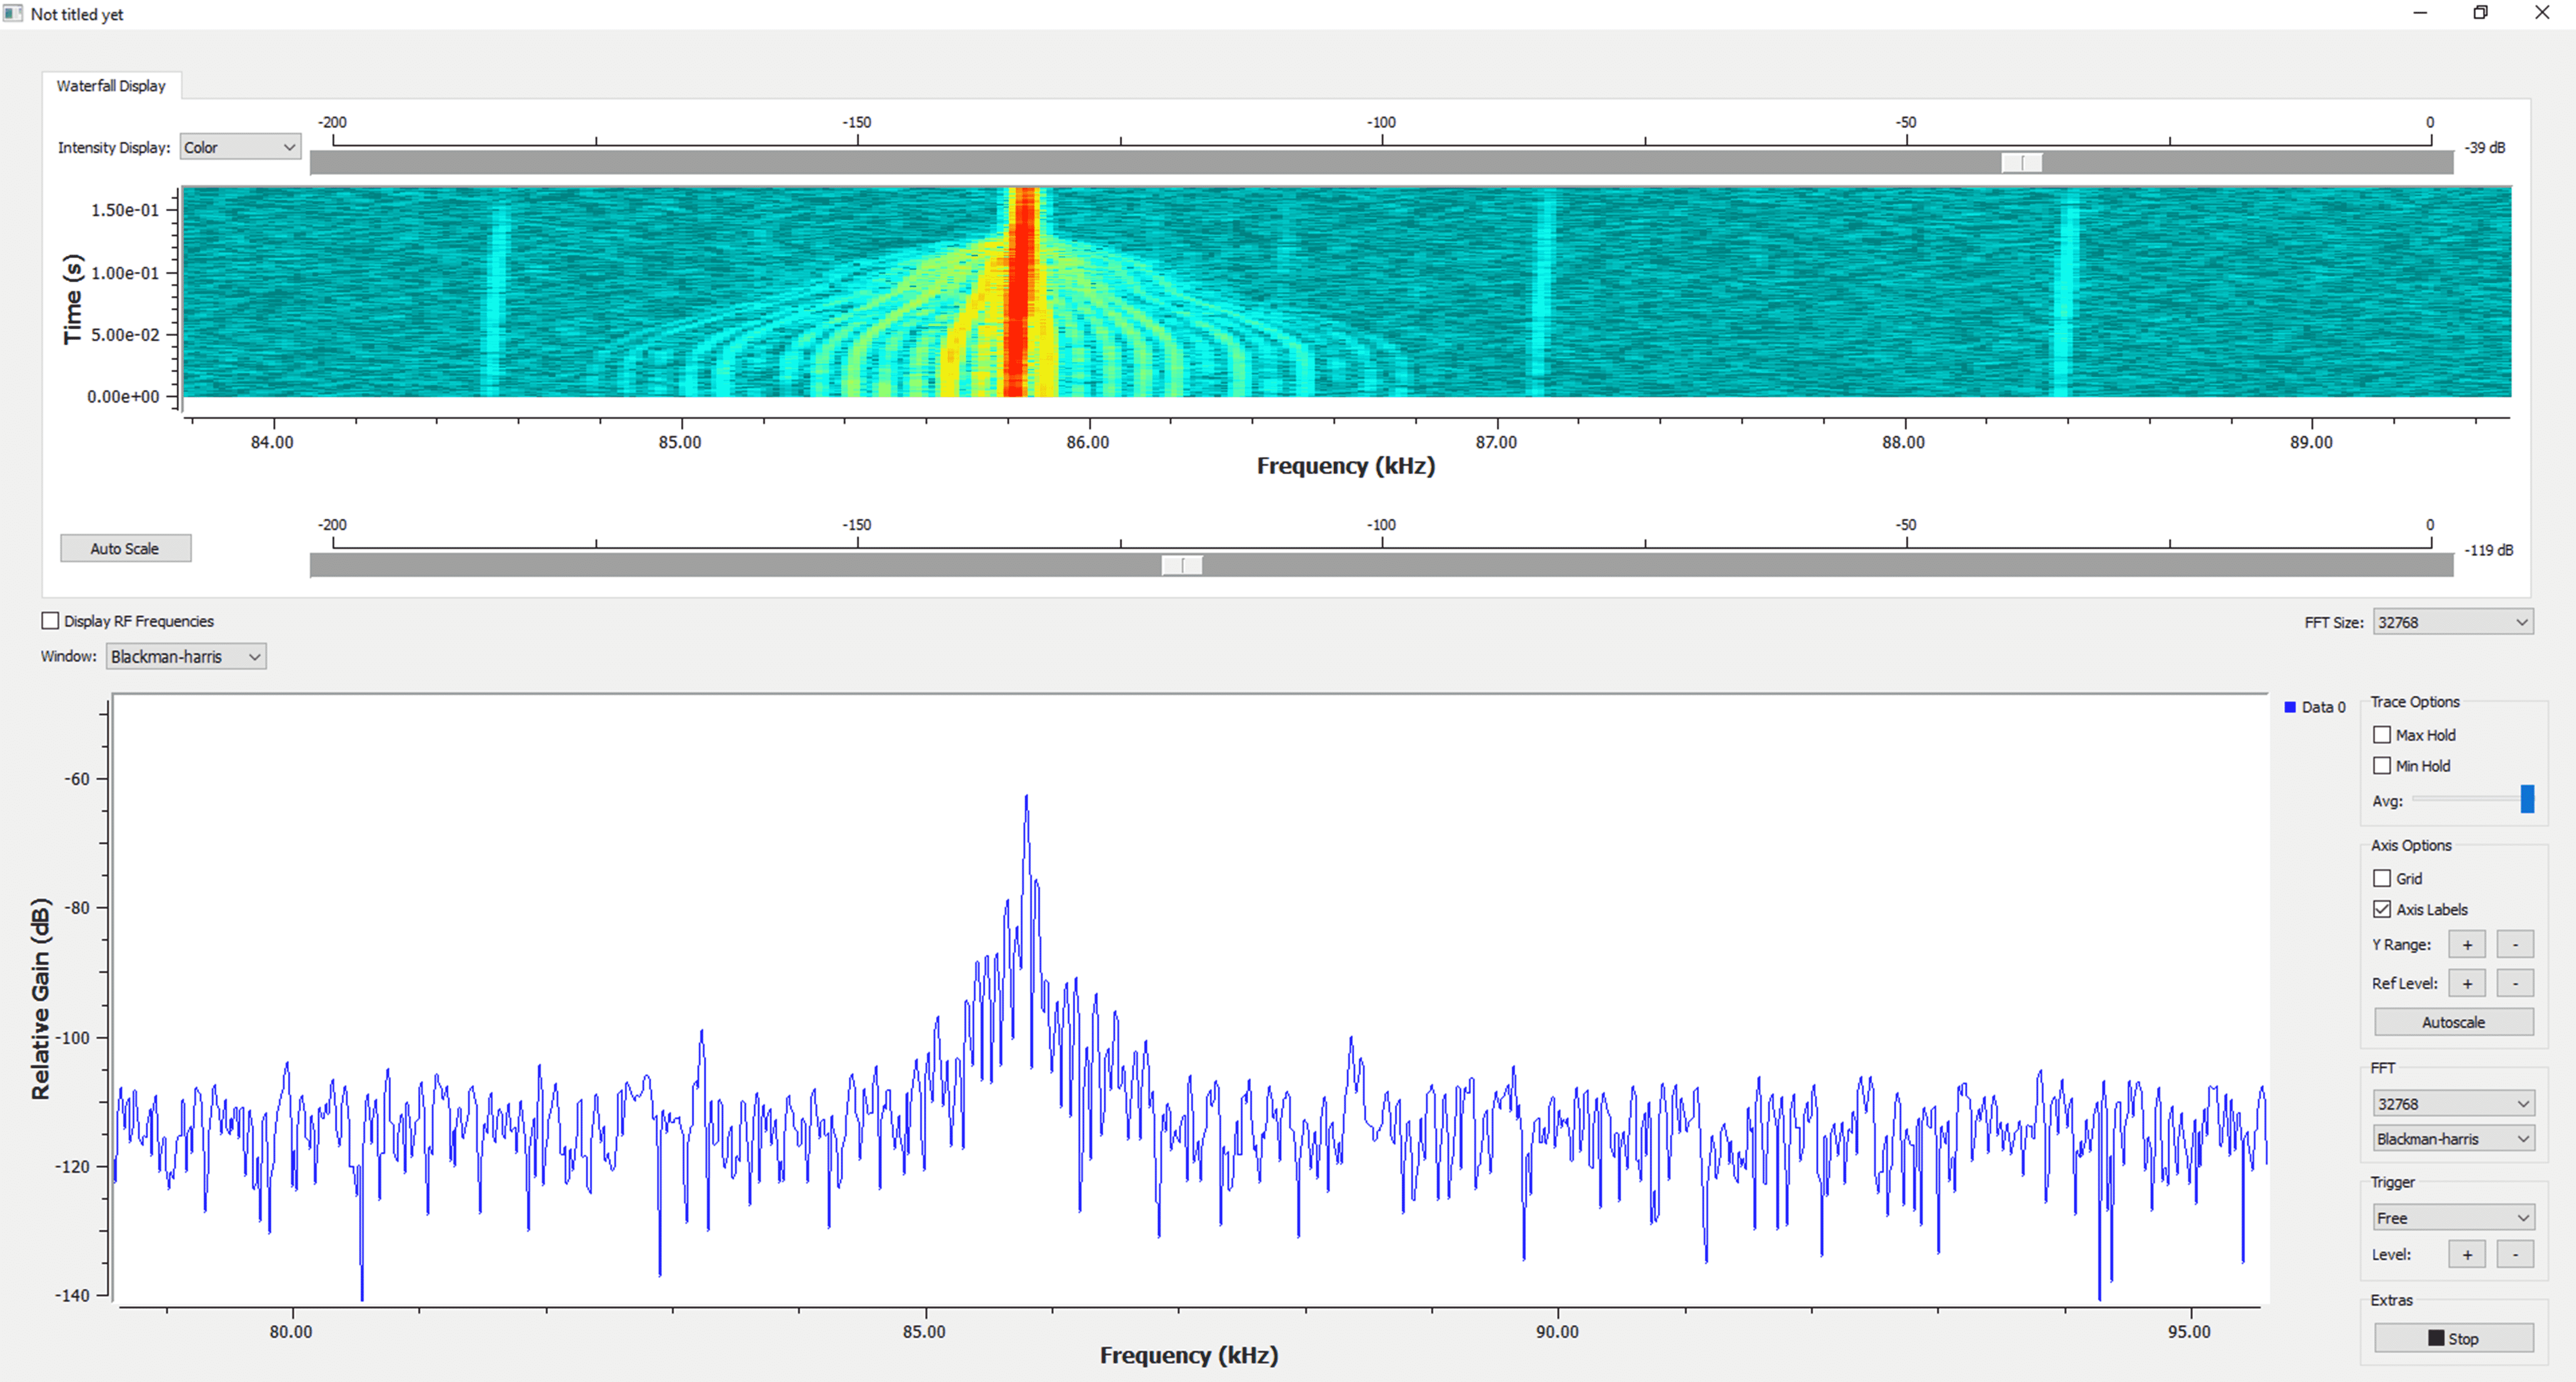
\includegraphics[width=\textwidth]{fan_off_to_high.png}
    \caption{Spectrum during the transition from off to high.}
    \label{fig:fan_off_to_high}
\end{figure}

\subsection*{Fan Slows from High to Low}
\begin{figure}[H]
    \centering
    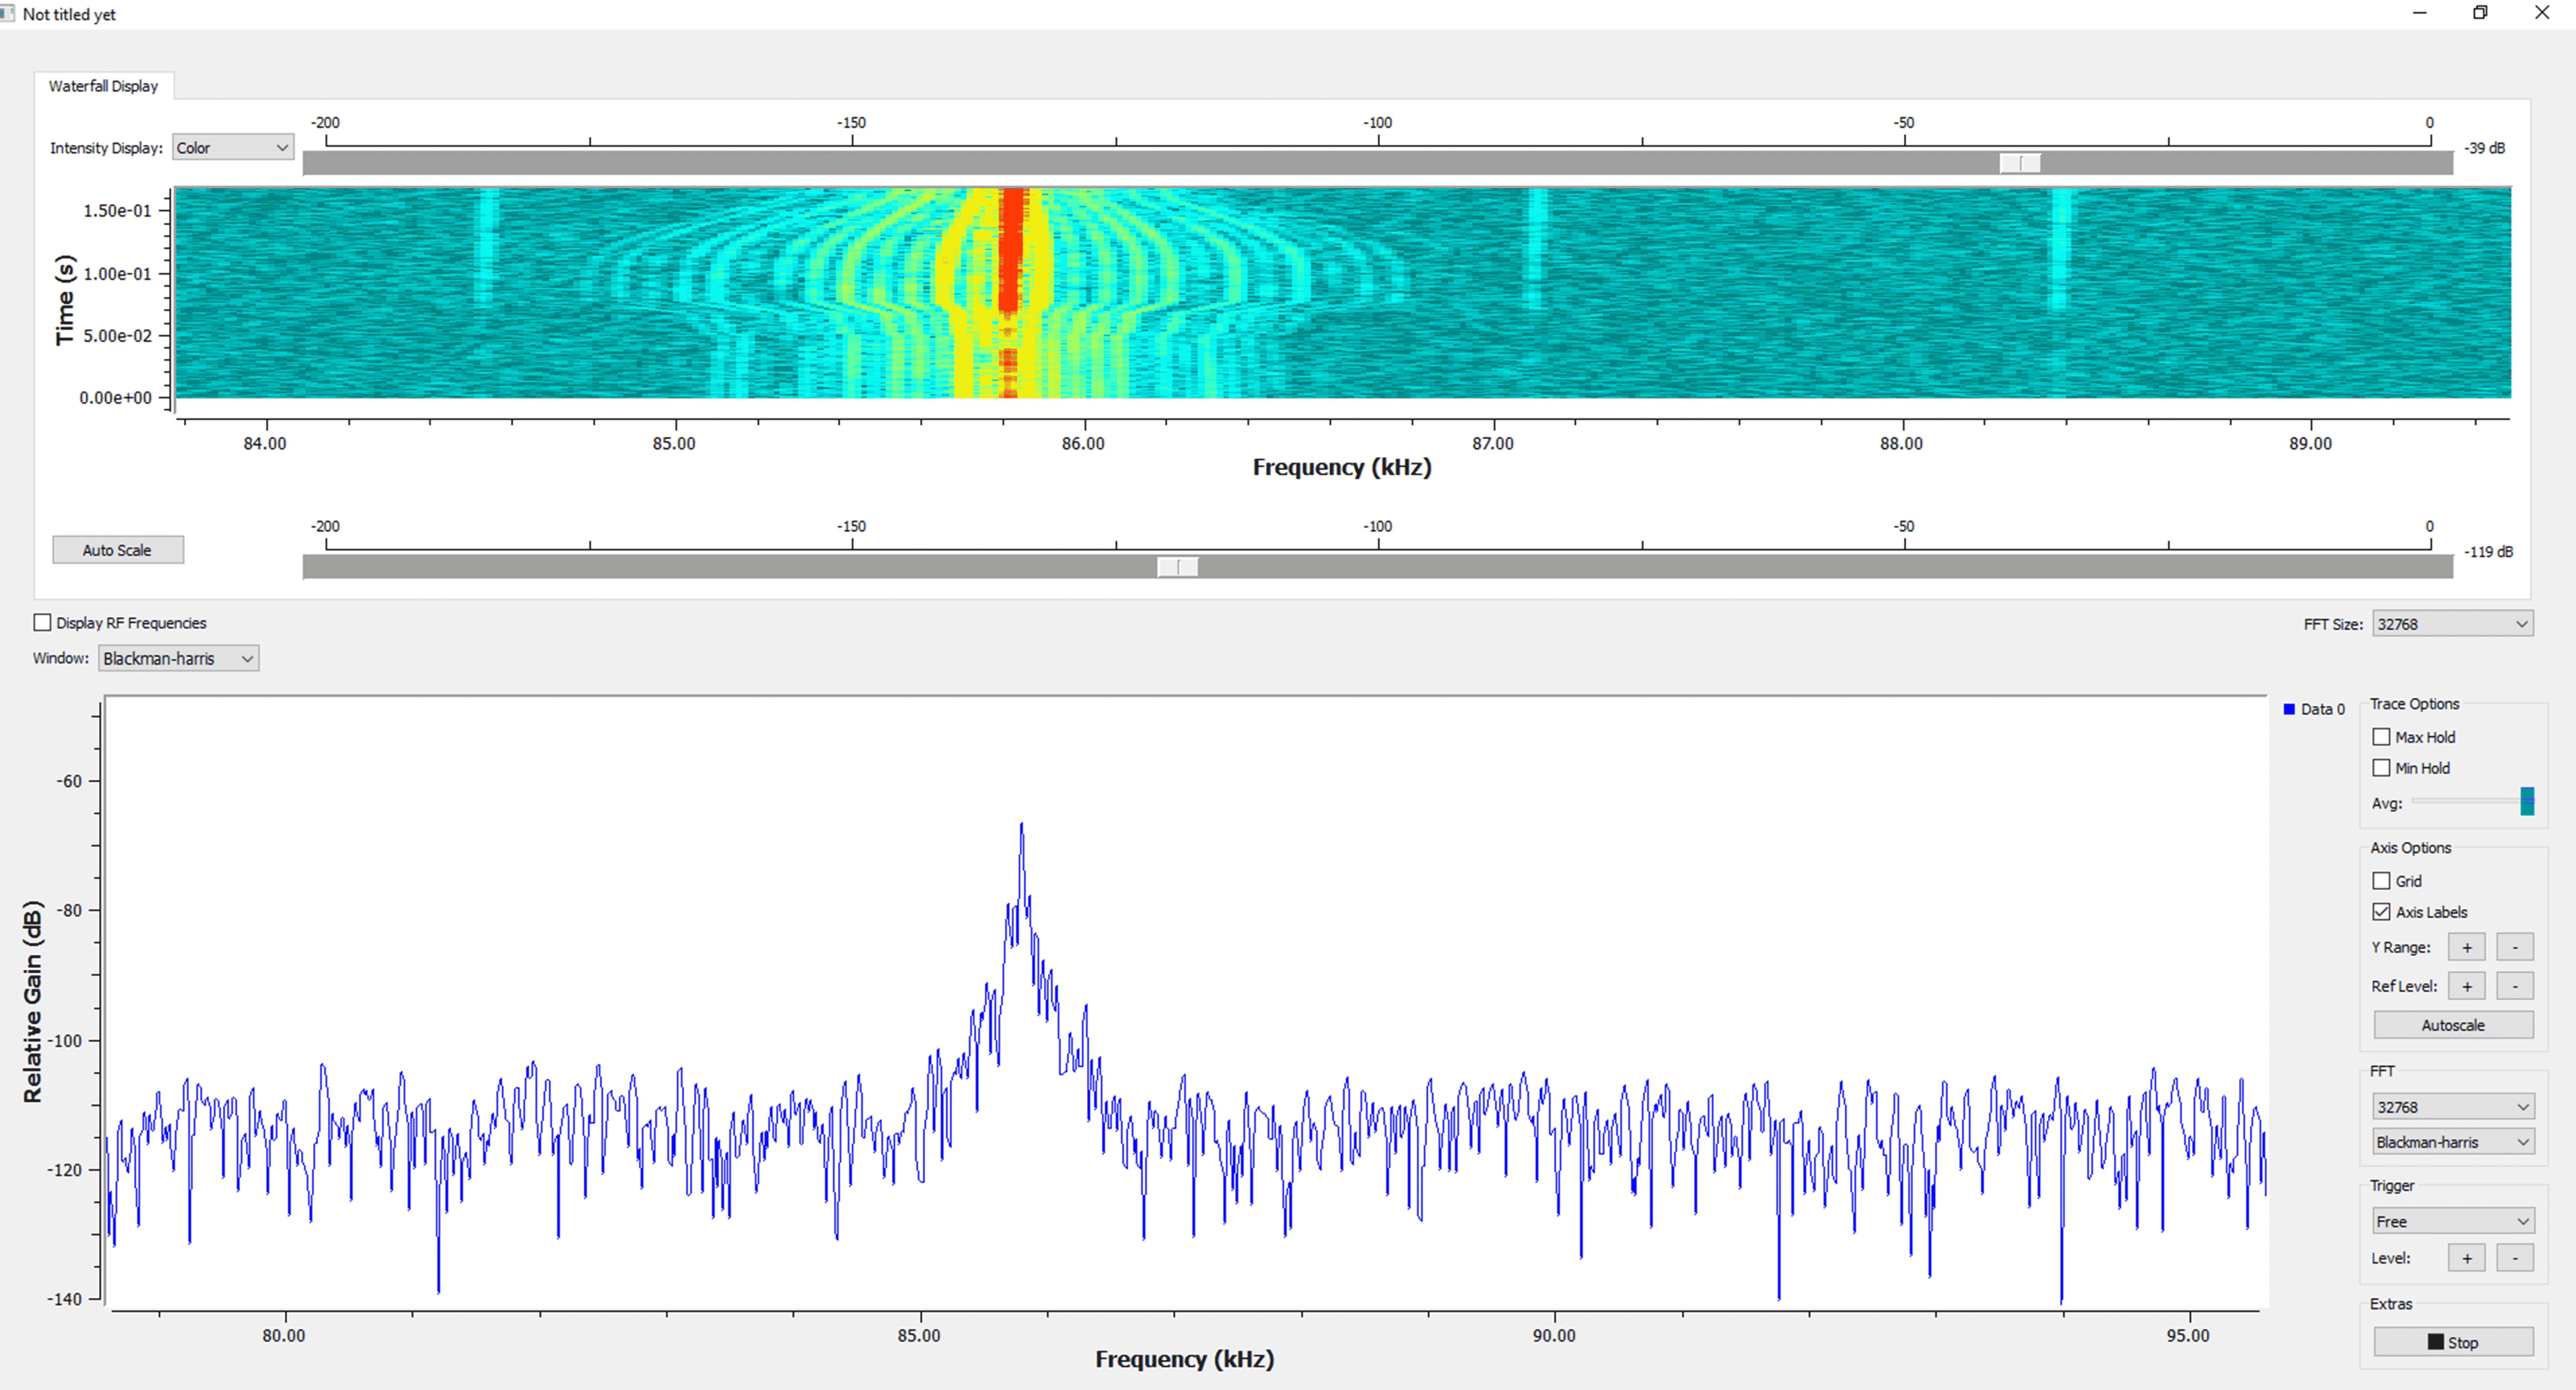
\includegraphics[width=\textwidth]{Fan_slows_from_hi_to_lo.png}
    \caption{Spectrum as the fan slows down from high to low.}
    \label{fig:fan_slows_from_hi_to_lo}
\end{figure}

\subsection*{No Fan Interference}
\begin{figure}[H]
    \centering
    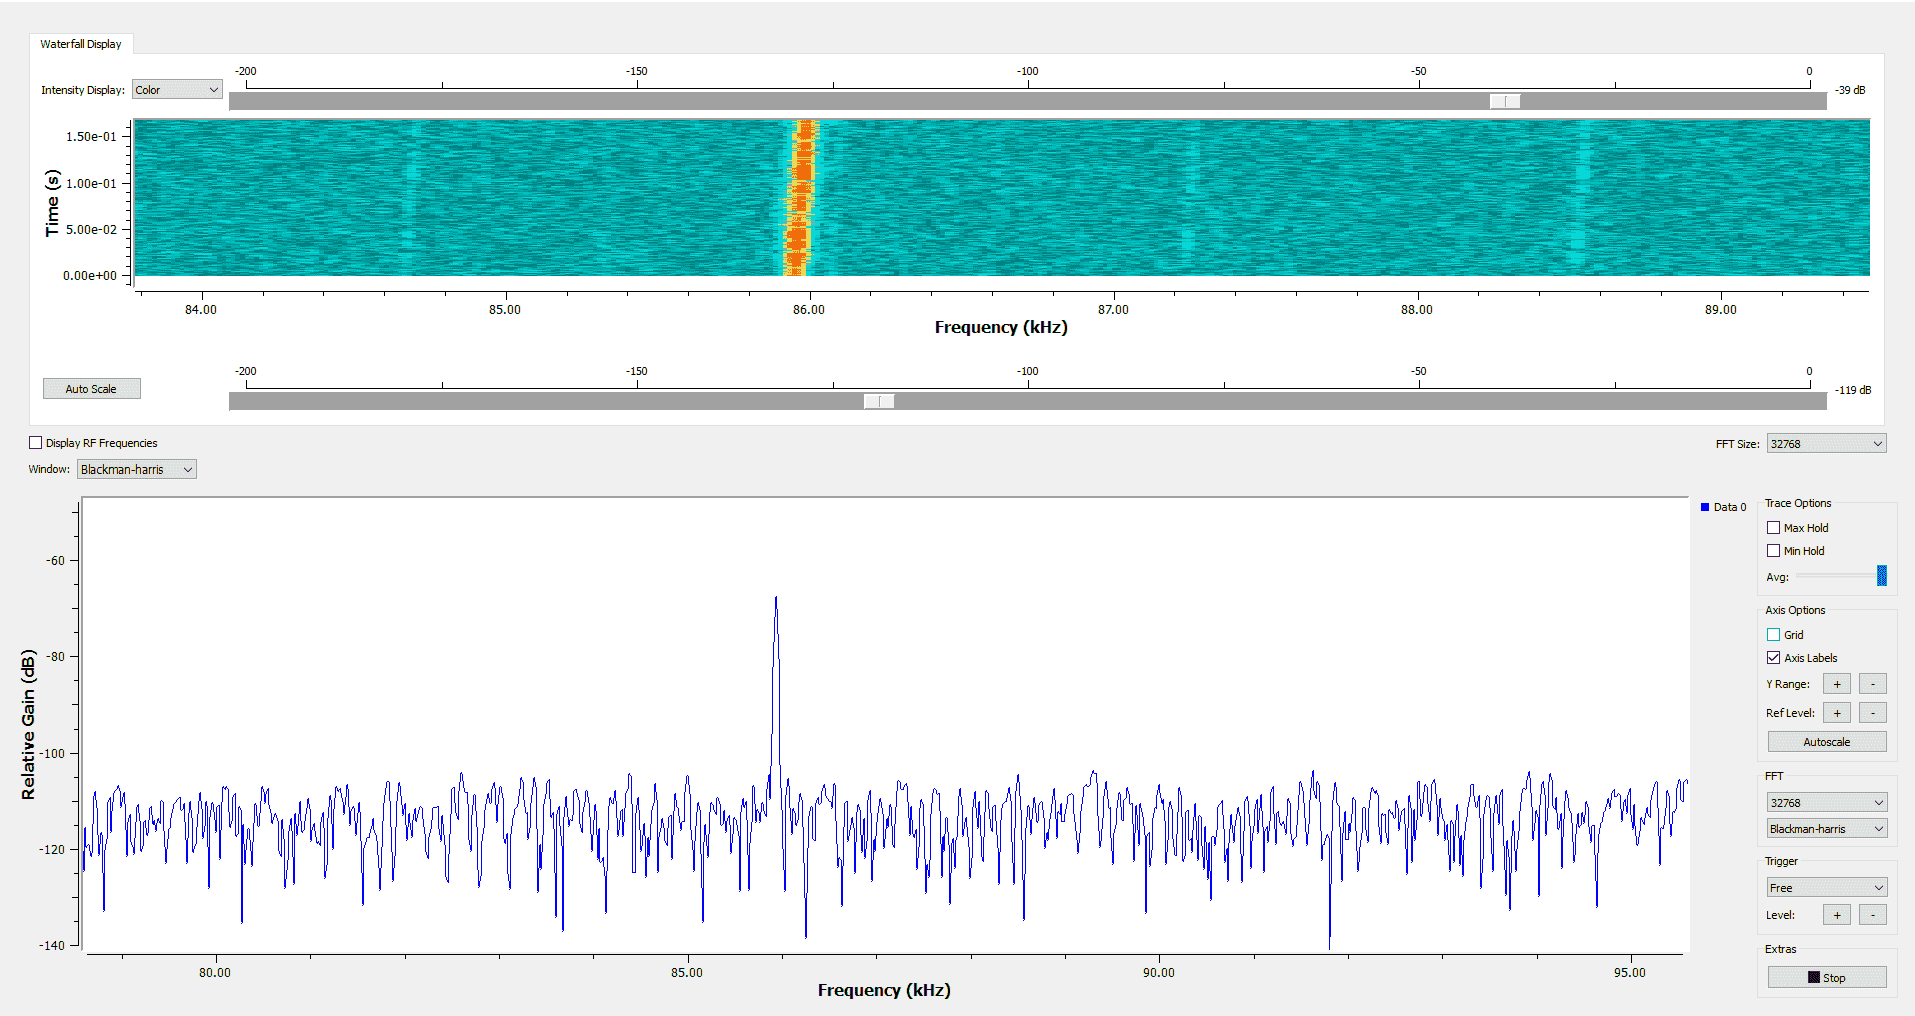
\includegraphics[width=\textwidth]{no_fan.png}
    \caption{Spectrum with no fan interference, alternate view.}
    \label{fig:no_fan_alt}
\end{figure}




\appendix
\section{MATLAB Code for Transmitter}
The MATLAB code used for the transmitter part of the experiment is listed below:
\lstinputlisting[language=Matlab]{pluto_transmitter_multiPathExperiment_toBeCompleted.m}

\section{MATLAB Code for Receiver}
The MATLAB code used for the receiver part of the experiment is listed below:
\lstinputlisting[language=Matlab]{pluto_receiver_multiPathExperiment_toBeCompleted.m}


\end{document}
